
%(BEGIN_QUESTION)
% Copyright 2006, Tony R. Kuphaldt, released under the Creative Commons Attribution License (v 1.0)
% This means you may do almost anything with this work of mine, so long as you give me proper credit

Noen strømningsmålere for gasstrømmer bruker en datamaskin til å behandle data fra en differansetrykktransmitter (koblet over en orifise), en absolutttrykktransmitter (måler oppstrøms gasstrykk i røret), og en RTD (måler temperaturen til gassen):

$$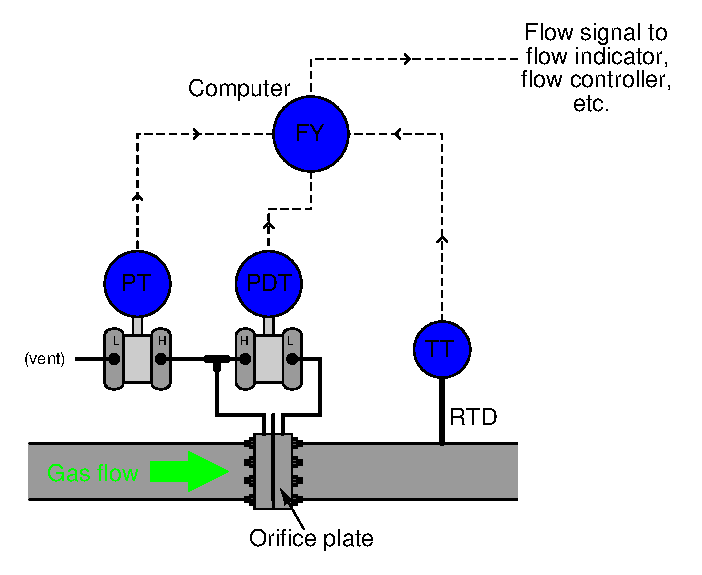
\includegraphics[width=15.5cm]{i00531x01.eps}$$

Én produsent lager en ``multivariabel'' transmitter som integrerer alle disse komponentene i én enhet:

$$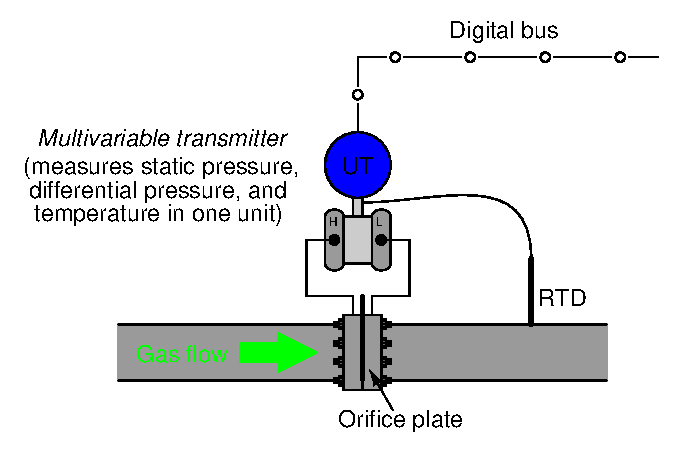
\includegraphics[width=15.5cm]{i00531x02.eps}$$

Hva er hensikten med dette? Hvorfor er ikke en enkel differansetrykktransmitter koblet over orifiseplaten god nok for strømningsmåling?

\vskip 20pt \vbox{\hrule \hbox{\strut \vrule{} {\bf Forslag til sokratisk diskusjon} \vrule} \hrule}

\begin{itemize}
\item{} Forklar hvorfor denne formen for ``kompensert'' gasstrømningsmåling egner seg godt for \textit{custody transfer}-applikasjoner.
\item{} I custody transfer-applikasjoner er det normalt tre parter som er interessert i transaksjonen: kjøper, selger og myndigheter. De to første er åpenbare, men hvorfor har myndighetene interesse i kalibreringsnøyaktigheten til instrumentet?
\end{itemize}

\underbar{file i00531}
%(END_QUESTION)





%(BEGIN_ANSWER)

Når det statiske trykket og/eller temperaturen i gasstrømmen endres, vil tettheten påvirkes. Dette gir igjen en ikke-lineær effekt på sammenhengen mellom differansetrykk og strømning for orifiseplaten. Ved å måle statisk trykk og temperatur, og deretter behandle disse dataene i en datamaskin sammen med differansetrykkmålingen, kan man få sann volumstrøm (``standard'' kubikkfot per minutt) eller massestrøm (pund per minutt).

\vskip 10pt

Slike trykk- og temperaturkompensasjoner er heller ikke begrenset til elektroniske instrumenter. Jeg har selv sett både turbinmålere og fortrengningsmålere med innebygde mekanismer for statisk trykk- og temperaturkompensasjon for nøyaktig måling av naturgass. Siden dette er en custody transfer-applikasjon (måling av gassmengde levert fra leverandør til betalende kunde), er nøyaktighet avgjørende for at begge parter skal få en ``rettferdig avtale.''

\vskip 10pt

AGA (American Gas Association) sin AGA-3-standard for gassmåling med orifiseplate ser slik ut:


$$Q_v = F_n (F_c+F_{sl}) Y_1 F_{pb} F_{tb} F_{tf} F_{gr} F_{pv} \sqrt{P_{f1} \Delta P}$$

\noindent
Der,

$Q_v$ = Volumstrøm

$F_n$ = Numerisk konverteringsfaktor (for å ta hensyn til måleenheter)

$C_d$ = Utløpskoeffisient (lik $F_c + F_{sl}$)

$F_c$ = Orifiseberegningsfaktor

$F_{sl}$ = Helningsfaktor

$Y_1$ = Ekspansjonsfaktor basert på oppstrøms tapping

$F_{pb}$ = Trykk-basisfaktor, satt til 1.0 ved 14.73 PSIA

$F_{tb}$ = Temperatur-basisfaktor, satt til 1.0 ved 60$^{o}$ F

$F_{tf}$ = Strømmende temperaturfaktor

$F_{gr}$ = Spesifikk gravitasjonsfaktor

$F_{pv}$ = Superkompressibilitetsfaktor

$P_{f1}$ = Absolutt strømmende trykk basert på oppstrøms tapping

$\Delta P$ = Differansetrykk over orifise, tommer H$_{2}$O ved 60$^{o}$ F

%(END_ANSWER)





%(BEGIN_NOTES)


%INDEX% Måling, strømning: trykk- og temperaturkompensasjon for orifiseplate

%(END_NOTES)

